
\section{Introduction}
\label{sec:intro}
The friends-of-friends (FOF) algorithm can be used to identify halos from N-body simulations. These halos provide information to analyze structure formation, galaxy formation and the content of the universe. A particularly important step in halo analysis is to determine the halo centers which can be used to compute mass functions and compare simulation results with observations. 
Analyzing halos' statistics can be very time consuming and computationally demanding mainly due to the large number of particles included in the halos. In modern cosmology simulations, a typical halo can use hundreds of millions of particles.  

One common definition of the halo center is the ``most bounded particle'' (MBP) which is the particle within a halo with the lowest potential. The potential of a given particle is computed as the sum over all other particles of the negative of mass divided by the distance.  
 \[ MBP=\min_i \ds\sum_{j\neq i}\frac{-m_j}{d(X_i,X_j)}\]
 where $X_i$ is the $i$-th particle, $m_i$ is its corresponding mass, and $d(X_i,X_j)$ is the Euclidean distance between particles $X_i$ and $X_j$. Another type of halo center is the ``most connected particle'' which is the particle within a halo with the most ``friends'', see Figure \ref{mbp_mcp}. In this work, we will focus on finding MBP. The most straightforward way to calculate MBP is to simply compute the potential for each particle and then take the minimum (see Algorithm \ref{Naive}), which requires $O(N_p^2)$ operations, where $N_p$ is the number of particles in the halo. Figure\ref{fig:naive} illustrates where MBP can be in a given halo. Variations have been designed to accelerate the brute force performance. For example, in \cite{fasel2011cosmology}, a $A^{*}$ search algorithm has been used to approximate the potentials and showed eight times faster than brute force algorithm. Another approach is to utilize binning algorithm to rule out the particles which can not be MBP so that to reach a complexity of $O(mN_p)$, however, for most of the times, $m$ can be still very large. 

 
 One common feature of the existing approaches is that the BP is exactly calculated. We notice that the BP map of a halo is smooth in the sense of small value change around neighborhood (shown in Figure \ref{fig:naive}). Therefore, in this work, instead of exact calculation, we will take advantage of this property and design a hierarchical algorithm to approximate BP based on neighborhood information, so to dramatically accelerate the MBP finding. 
\begin{figure}[H]
\centering
\label{mbp_mcp}
    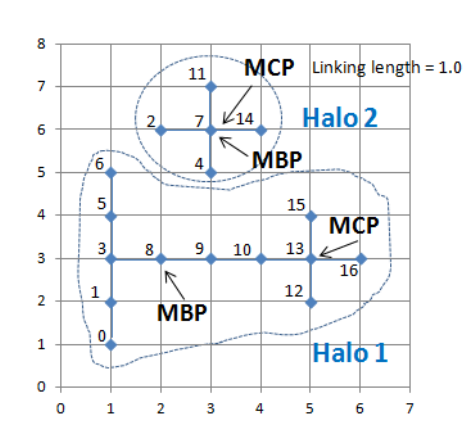
\includegraphics[scale=0.7]{MBP_MCP.png}
    \caption{Illustration of MBP and MCP on halos}
\end{figure}
 \begin{algorithm}
\caption{Naive}
\label{naive}
\begin{algorithmic}[1]
  \State $\ds MBP=\min_i \ds\sum_{j\neq i}\frac{m_j}{d(X_i,X_j)}$
\end{algorithmic} 
 \end{algorithm}
\begin{figure}[H]
\centering
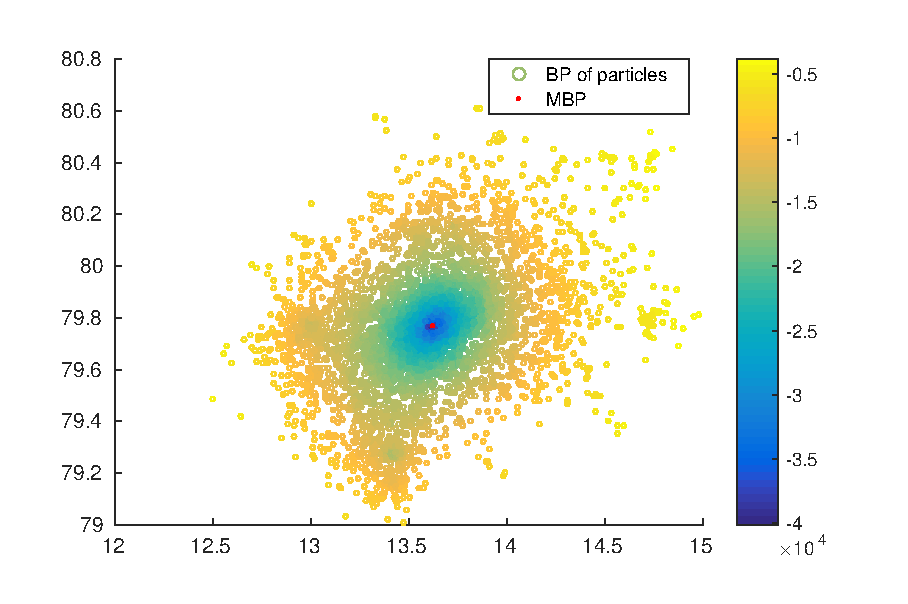
\includegraphics[scale=0.45]{naive}%
\caption{MBP Illustration}
\label{fig:naive}
\end{figure}
\section{Algorithm}
We first observe that the potential map from every particle is relatively smooth in its local region. Therefore, our approach is to approximate the potential map by a few sampled particles, and gradually narrow down to a small region where the MBP can be. In the other word, we approximate the BP only by the particles in a certain neighborhood. Therefore, an essential step is to perform a range search. We first use kdtree to construct the neighboring information among particles. kd tree is a data structure by partitioning the space through alternative dimension for organizing points in a k-dimensional space. This structure is only constructed once in the beginning. Throughout the process, the pre-constructed structure will be used for range which searches for ranges at a given distance parameter. For example, if a tree is storing values corresponding to distance, then a range search is to look for all members of the tree which in the distance smaller than the given threshold. Since k-d trees divide the range of a domain in half at alternative dimension at each level of the tree, they are efficient for performing range searches.  

Once the kdtree is constructed, we first uniformly sample a few seeding particles, approximate their BPs by the range search at a given distance threshold as $\varepsilon$. Then we interpolate the coarse BP map for every particle, use a peak finding algorithm to locate the points with the first few smallest BPs. Meanwhile, we mark the particle with the smallest BP as a temporary MBP. Next, we start range search on the newly selected seedling particles with the smallest BPs. From this step, instead of only approximating BPs for the seedling particles, we approximate BPs for every particle in the ranges, repeat the steps of interpolating, peak finding, and locate temporary MBP until the current temporary MBP coincides with the previous temporary MBP. The full algorithm is described as follows: 
\begin{algorithmic}[h]
\Procedure {$MBP=recursive\_localMBP(X,m)$}{}
\State{tree=kdtree(X).}
\State {\bf If $(level=1)$}
\State Select uniformly distributed random indices $\tilde{i}$ from $[1,\dots,N_p]$ as $Seeds$.
\State For each $\tilde{i}$, $IDX=rangesearch(tree,X_{\tilde{i}},\varepsilon)$, where $\varepsilon$ is the neighborhood radius provided for tree search, and $IDX$ is the index function to indicate which particles are friends of $X_{\tilde{i}}$. Calculate $\tilde{BP}_{\tilde{i}}=\ds\sum_{\{j|IDX\neq j\}}\frac{-m_j}{d(X_{\tilde{i}},X_j)}$, where $\tilde{BP}$ denotes local bounded potential. 
\State Update $Seeds$ as local peaks of the $\tilde{BP}$ map, and find $\tilde{MBP}$ as the minimum of $\tilde{BP}$ map. 

\State {\bf Else}

\State for each $\tilde{i}$ in $Seeds$, calculate $IDX_{\tilde{i}}=rangesearch(tree,X_{\tilde{i}},\tilde{\varepsilon})$.

\State Calculate $\tilde{BP}$ for each particle in $IDX_{\tilde{i}}$ for each $\tilde{i}$.
\State Set $\tilde{MBP}_0=\tilde{MBP}$.
\State Find $\tilde{MBP}$ as the minimum of $\tilde{BP}$ map. 
\State if $\tilde{MBP}_0=\tilde{MBP}$, stop the procedure; else, $level=level+1$.
\EndProcedure
\end{algorithmic} 

The range search parameter is chosen based on a simple numerical test to find a reasonable value so that the approximated BP is agreeing well with the exact BP as shown in Figure \ref{rsthreshold}.

\begin{figure}[ht]
\centering
    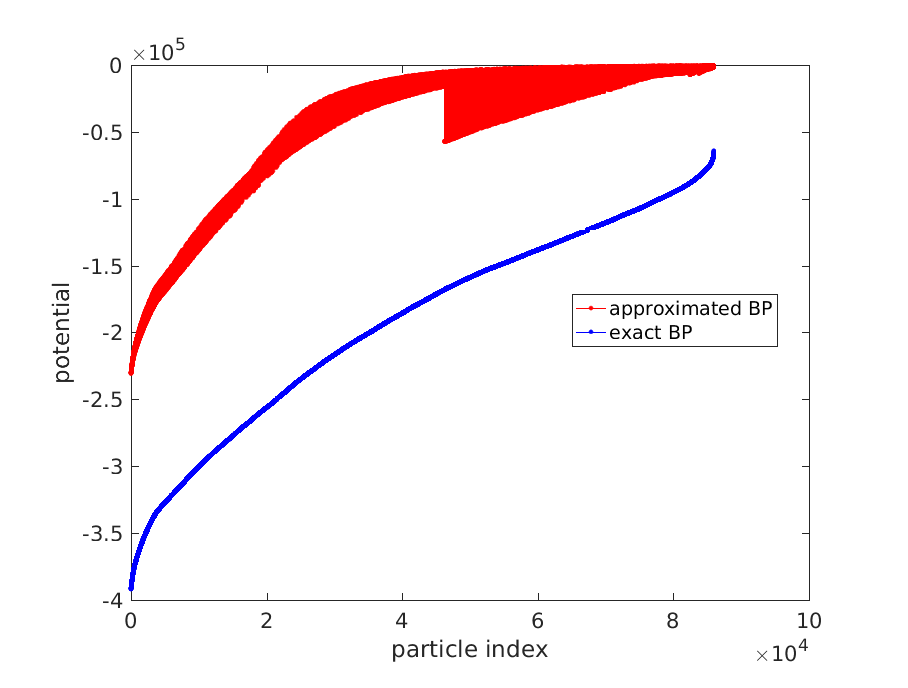
\includegraphics[scale=0.5]{localVSglobal}
    \caption{Given the range search parameter we used through every numerical test,  we illustrate here the local BPs have the similar shape as the global BPs which makes them share the common minimum.}
    \label{rsthreshold}
\end{figure}


\section{Complexity Analysis}
In this section, we estimate the complexity of our proposed algorithm. Each level performs the following computations:
\begin{itemize}
  \item Range search: $O(N_p)$. 
  \item Approximate local BP: $O(n^2)$ where $n$ is roughly the number of particles in the range.
  \item Peak finding: the dominant calculation is sorting which takes $O(nlogn)$. 
\end{itemize}
In average, it takes 3 levels to converge, we also choose to take the first 4 local minimum as seedings from level 2, then adding the complexity of one time kd-tree construction which is $O(N_p \logN_p)$, the total complexity is
\[\displaystyle O(N_p \log N_p)+3\left(O(N_p)+O(n\logn)+4O(n^2)\right)\] 
\section{Numerical Result}

We now show how the algorithm works on a relatively challenging 2D example in Figure \ref{illu_level} where the halo contains approximately 3 locally dense area. Therefore, in this example, there are 3 local minimums for MBP finding. Figure \ref{2d_result} shows the corresponding result where the approximated MBP agrees with the exact MBP.

Next, we run our algorithm on 500 simulated 3D dark matter halos. In Figure \ref{fig:timing}, we can see as the number of particles increases, the time elapsed for our proposed algorithm reduces about 20 times less the time elapsed for the brute force method. Meanwhile, Figure \ref{fig:error} shows the accuracy of our proposed algorithm compared to the brute force, the biggest error is on the order of $10^{-3}$ which in reality, if two particles have the distance shorter than $10^{-3}$, we do not distinguish these two particles. Therefore, the accuracy is achieved through our proposed algorithm as well.  

\begin{figure}[h]
\subfloat[ \label{fig:1st}]{
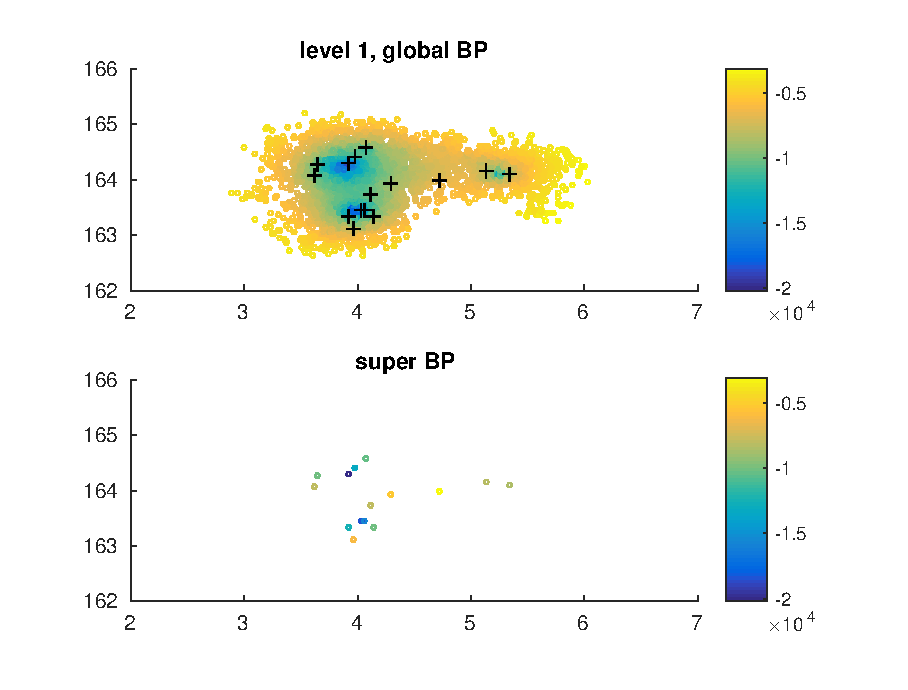
\includegraphics[scale=0.5]{2d_1}}
\hfill
\subfloat[ \label{fig:2nd}]{
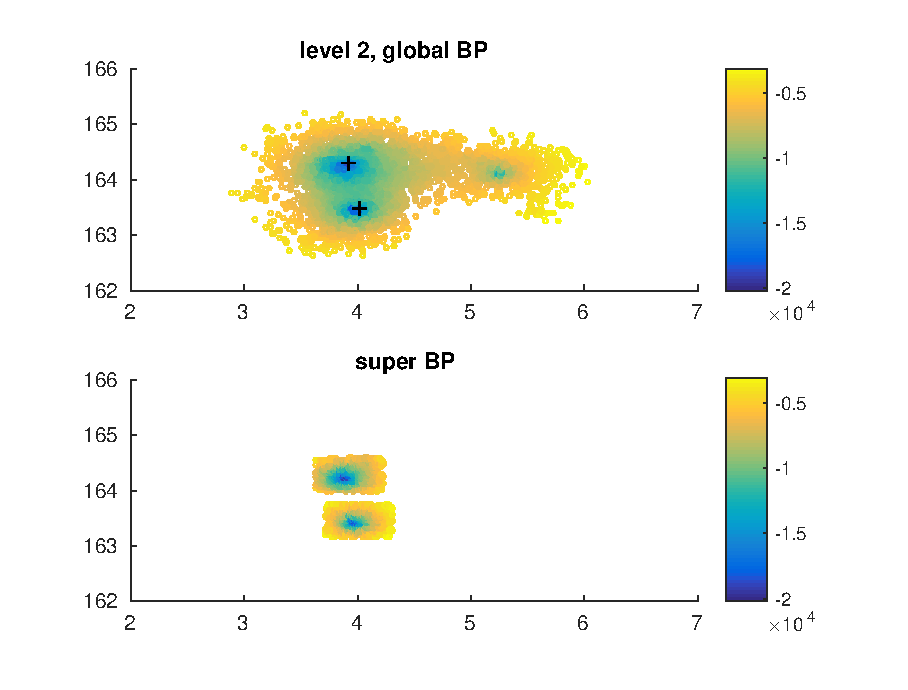
\includegraphics[scale=0.5]{2d_2}}
\caption{Demonstrate the recursive process}
\label{illu_level}
\end{figure}

\begin{figure}[ht]
\centering
    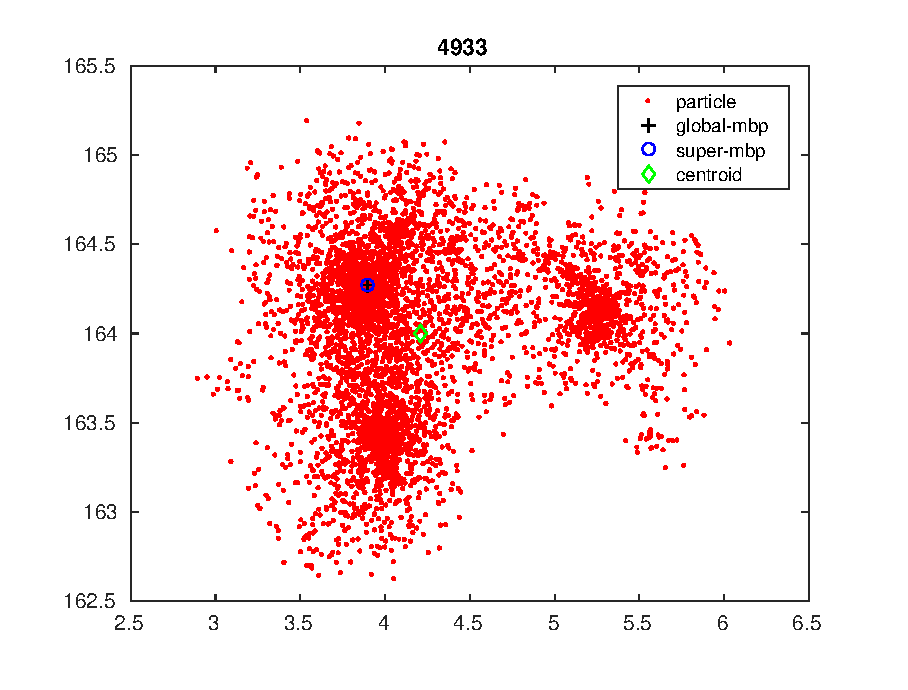
\includegraphics[scale=0.45]{2d_result}
    \caption{the approximated MBP agrees with the exact MBP, we also show where the centroid is in this case to demonstrate multiple dense areas in this particular 2D halo}
    \label{2d_result}
\end{figure}

\begin{figure}[h]
\subfloat[ \label{fig:timing}]{
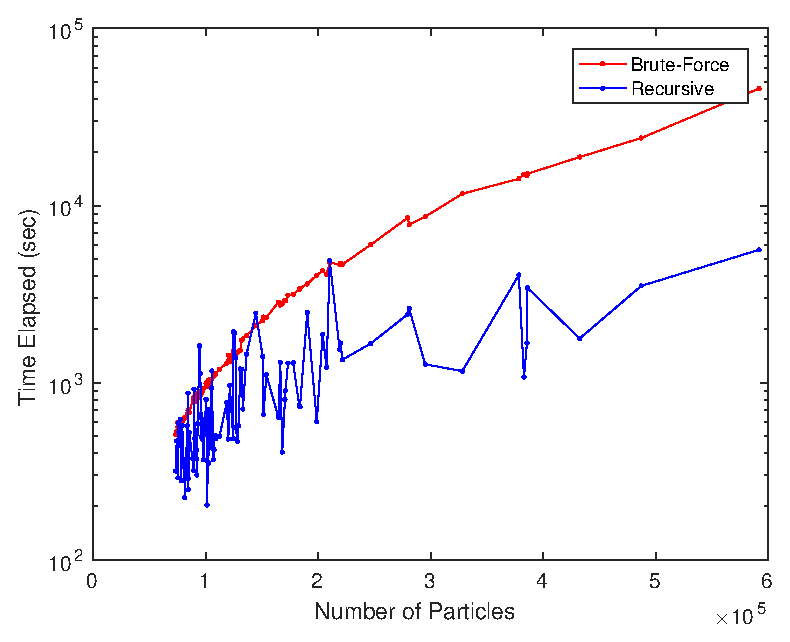
\includegraphics[scale=0.5]{3d_timing}}
\hfill
\subfloat[ \label{fig:error}]{
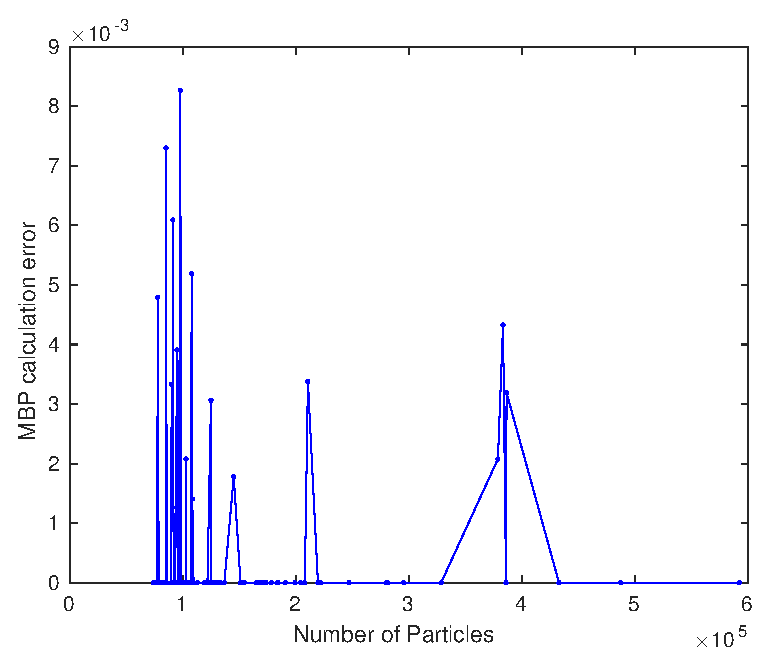
\includegraphics[scale=0.5]{3d_error}}
\caption{3D result}
\label{3dresult}
\end{figure}

% \section{Potential Variations}
%  \begin{algorithm}
% \caption{Mixed Particle/Super-particle Hierarchy}
% \label{sp-mixed}
% \begin{algorithmic}[1]
% \Procedure {$MBP=mixed\_kmeans(X,m)$}{}
% \State $[IDX,c]=kmeans(X,N_c)$, where $N_c$ is  the number of clusters, $IDX\in \mathbb{N}^{N_p}$ is the index function to indicate which cluster particle $X_i$ belongs to, ${\bf c} _i \in \R^{2}, \, i=1,\dots,N_c$ is the centroid of each cluster. 
% \State $\bar m_i=|\{j | IDX(j)=i\}|,\,\forall i=1:N_c$
% \State $SBP_i=\ds\sum_{\{j|IDX(i)\neq j\}}\frac{\bar m_j}{d(X_i,c_j)}+\ds\sum_{\{j|IDX(j)=IDX(i),i\neq j\}}\frac{m_j}{d(X_i,X_j)},\, \forall i$ 
% \State $MBP=\ds\min_i SBP_i$
% \EndProcedure
% \end{algorithmic} 
%  \end{algorithm}
% \begin{figure*}[t!]
% \centering
% \begin{subfigure}[t]{0.5\textwidth}
% \centering
% 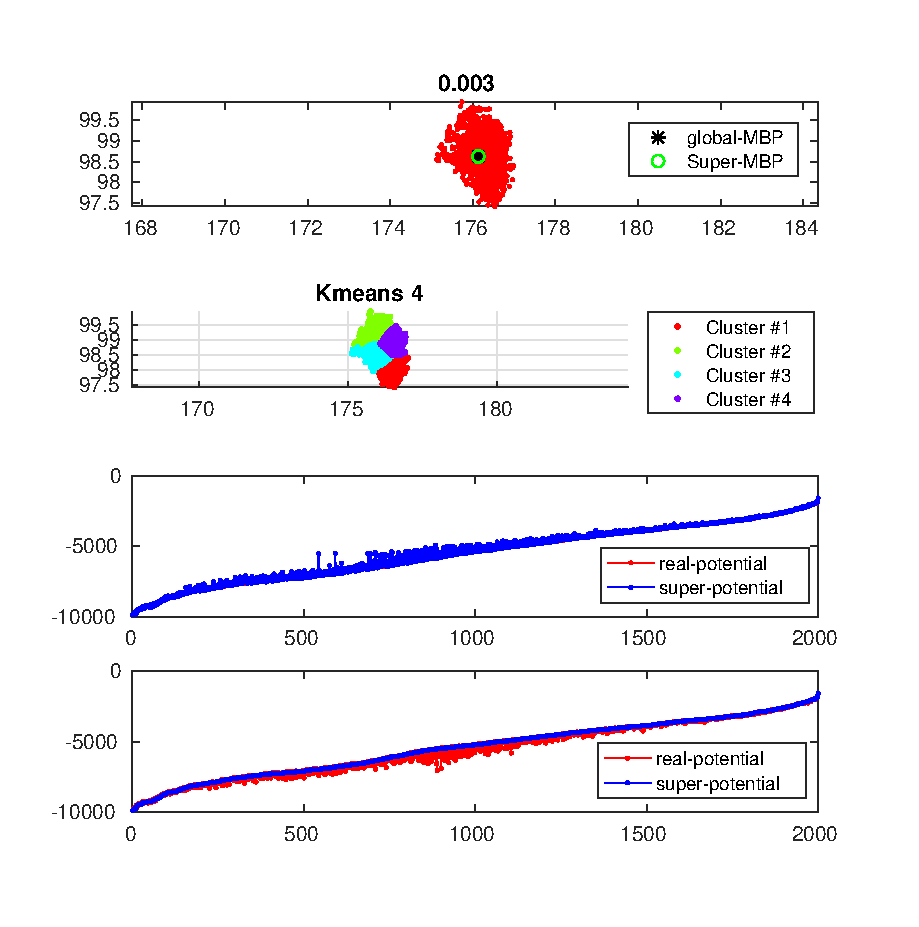
\includegraphics[scale=0.45]{sp_p_mixed_kmeans}
% \end{subfigure}%
% ~ 
% \begin{subfigure}[t]{0.5\textwidth}
% \centering
% 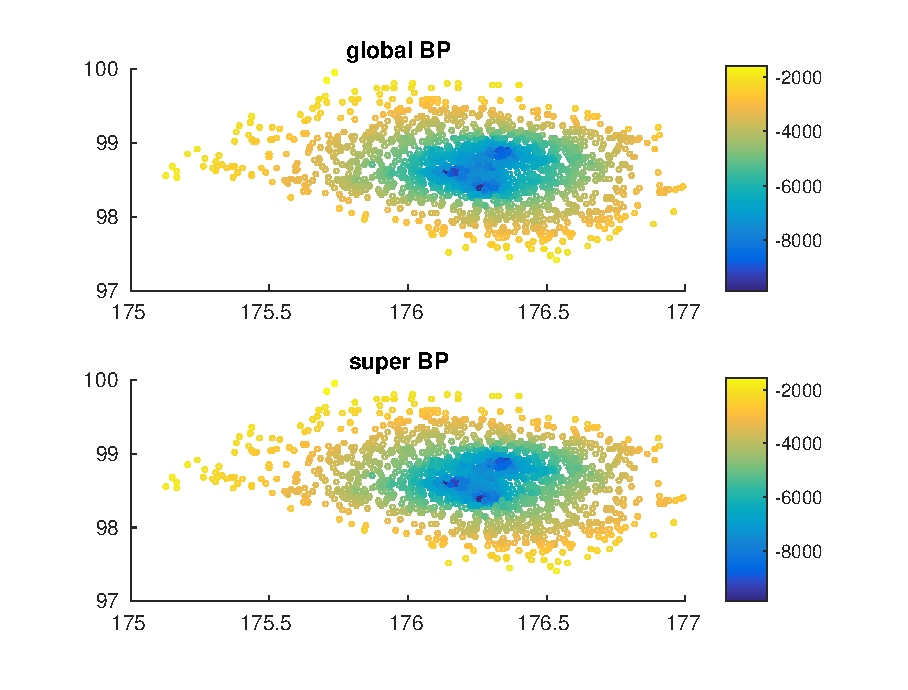
\includegraphics[scale=0.45]{sp_p_mixed_kmeans_bp}
% \end{subfigure}
% \caption{Result of Algorithm \ref{sp-mixed}}
% \end{figure*}
% 
%  \begin{algorithm}
% \caption{Super-particle Hierarchy}
% \label{sp-p}
% \begin{algorithmic}[1]
% \Procedure {$MBP=sp\_kmeans(X,m)$}{}
% \State $[IDX,c]=kmeans(X,N_c)$ 
% \State $\bar m_i=|\{j | IDX(j)=i\}|,\,\forall i=1:N_c$
% \State $MBP=\ds\min_i \ds\sum_{\{j|IDX(i)\neq j\}}\frac{\bar m_j}{d(X_i,c_j)}$ 
% \State $n_c=N_c$
% \State $k=1$
% \While{$k\leq n_k$}
% \State $MBP_{old} = MBP$
% \State $v=\{j\,|\,IDX(j)=IDX(MBP)\}$
% \State $[\tilde{IDX},\tilde{c}]=kmeans(X(i),\tilde{N_c}$
% \State $c=\{c_1,\dots,c_{MBP-1}\}\cup\tilde{c}_1 \cup \{c_{MBP+1},\dots,c_{N_c}\}\cup \{\tilde{c}_2,\dots,\tilde{c}_{\tilde{N_c}}\}\}$
% \State $IDX(v)=\tilde{IDX}+kN_c-1$
% \State $n_c=n_c-1+\tilde{N_c}$
% \State $\bar m_i=\frac{1}{|\{j | IDX(j)=i\}|},\,\forall i=1:n_c$
% \State $MBP=\ds\min_i \ds\sum_{\{j|IDX(i)\neq j\}}\frac{\bar m_j}{d(X_i,c_j)}$ 
% \If{$MBP=MBP_{old}$}
% \State Stop
% \EndIf
% \State $k=k+1$
% \EndWhile
% \EndProcedure
% \end{algorithmic} 
%  \end{algorithm}
% \begin{figure*}[t!]
% \centering
% \begin{subfigure}[t]{0.5\textwidth}
% \centering
% 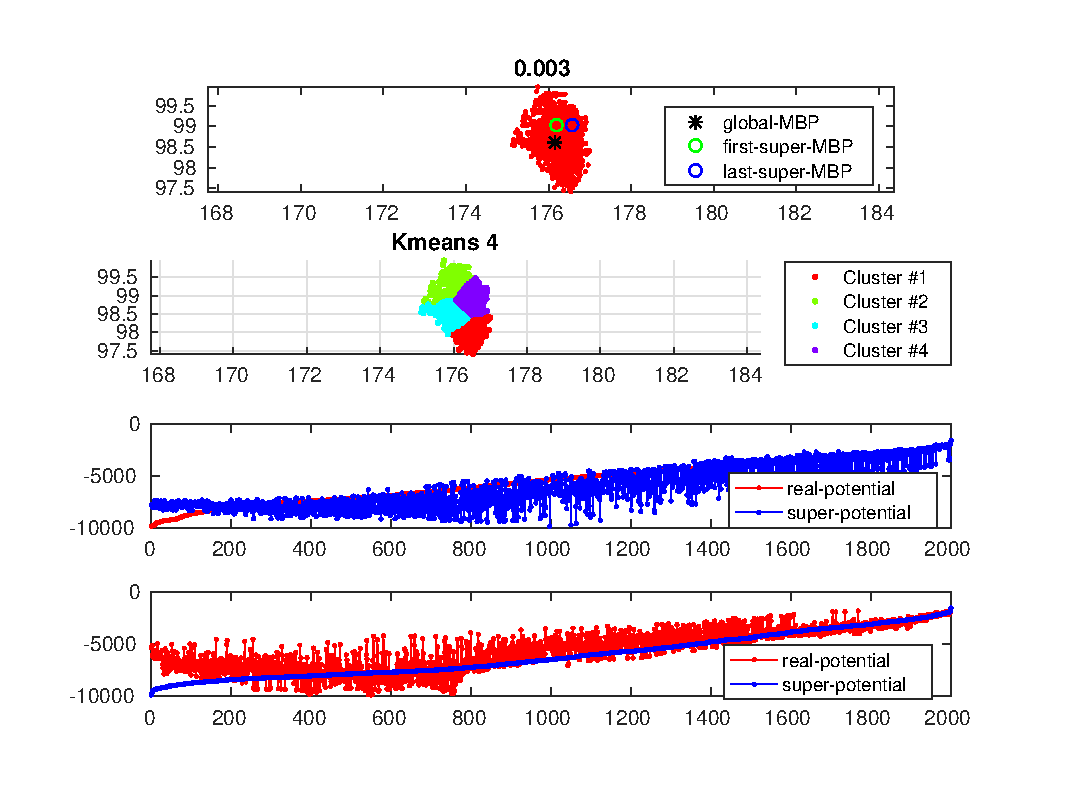
\includegraphics[scale=0.45]{sp_p_kmeans}
% \end{subfigure}%
% ~ 
% \begin{subfigure}[t]{0.5\textwidth}
% \centering
% \includegraphics[scale=0.45]{sp_p_kmeans_bp}
% \end{subfigure}
% \caption{Result of Algorithm \ref{sp-p}}
% \end{figure*}
% \begin{figure}[h]
% \centering
% 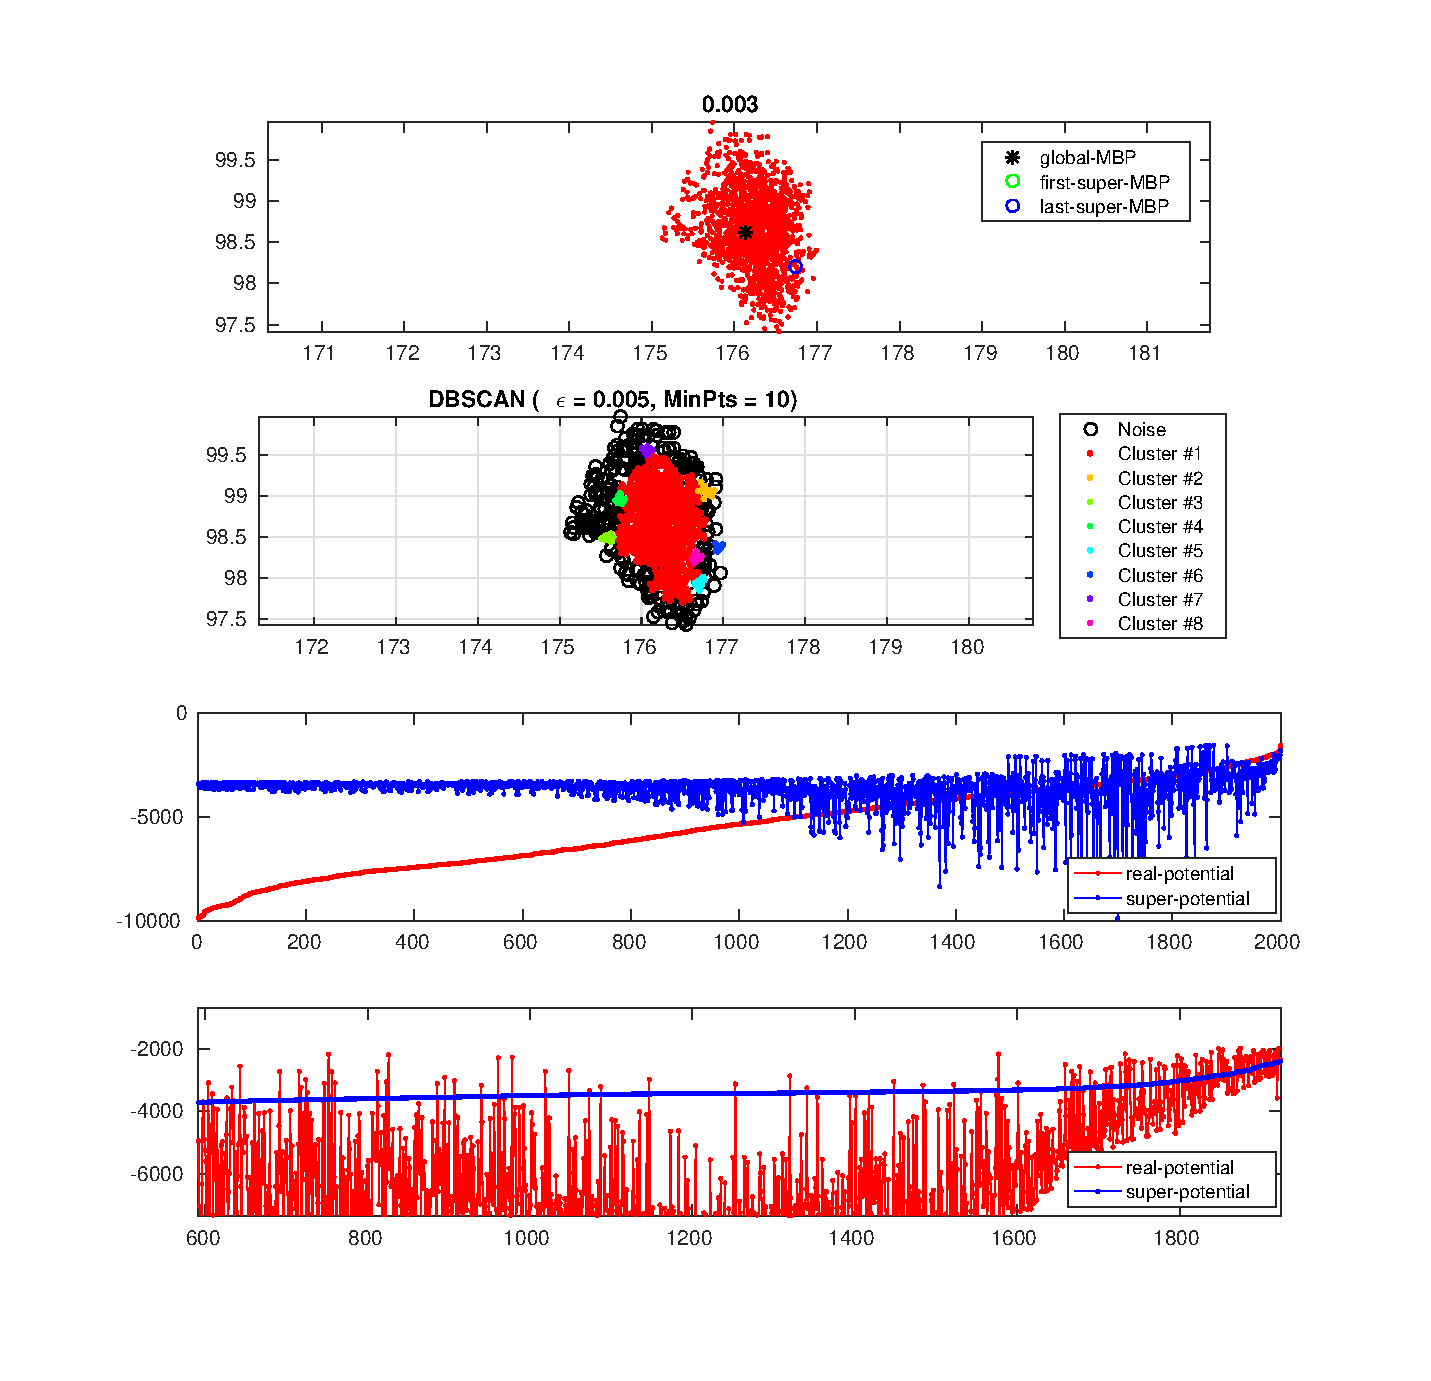
\includegraphics[scale=0.45]{sp_p_dbscan}%
% \caption{Result of replacing Kmeans by DBSCAN in Algorithm \ref{sp-p}}
% \label{fig:sp_dbscan}
% \end{figure}
% 
%  \begin{algorithm}
% \caption{Locate MBP from a subset of particles which forms the most dense super-particle via DBSCAN}
% \label{dbscan_max}
% \begin{algorithmic}[1]
% \Procedure {$MBP=mbp\_dbscan\_max(X,m)$}{}
% \State $[IDX,c]=dbscan(X,\varepsilon)$, where $\varepsilon$ is the linkage length provided for DBSCAN. 
% \State $\bar m_i=|\{j | IDX(j)=i\}|,\,\forall i=1:N_c$, where $N_c$ is the resulted number of clusters given $\varepsilon$
% \State $i_s=\ds\max_i \bar{m_i}$
% \State $V=\{j \,|\, IDX(j)=i_s\}$
% \State $SBP_i=\ds\sum_{i\neq j\}}\frac{m_j}{d(X_i,X_j)},\, \forall i\in V$ 
% \State $MBP=\ds\min_{i\in V} SBP_i$
% \EndProcedure
% \end{algorithmic} 
%  \end{algorithm}
% \begin{figure}[H]
% \centering
% 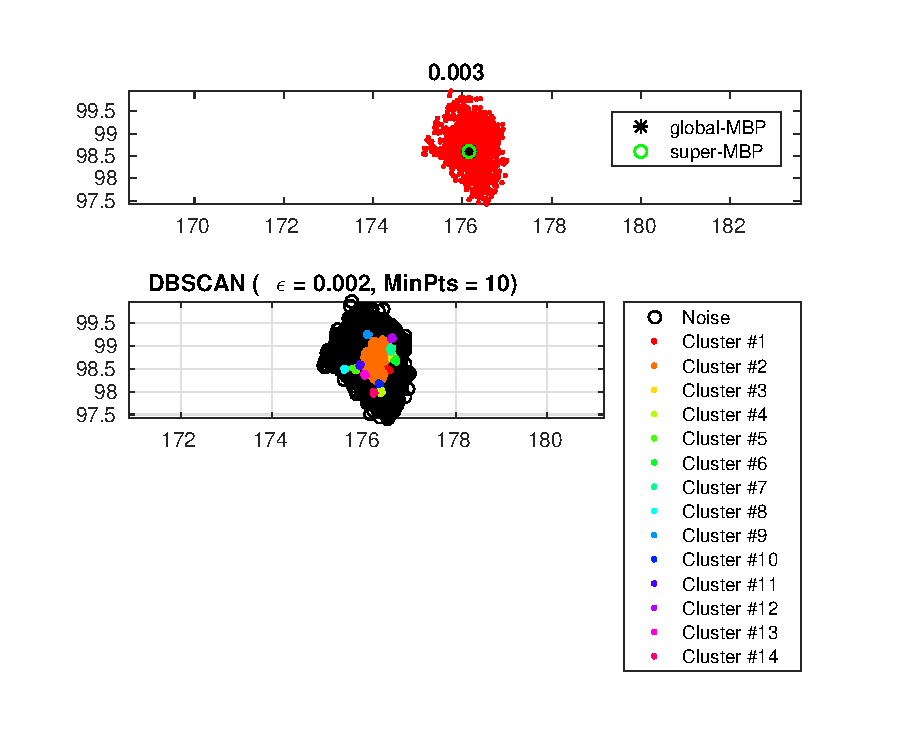
\includegraphics[scale=0.45]{p_dbscan_maxSub}%
% \caption{Result of Algorithm \ref{dbscan_max}}
% \label{fig:dbscan_max}
% \end{figure}

\section{Conclusion and Future Work}
We proposed a partially hierarchical framework to approximate MBP instead of exact calculation. The numerical result shows dramatic speedup comparing to the most common approach. However, there are still great potentials to further accelerate the performance. The first component to further explore is to shrink the range search parameter along each level. Intuitively, bigger the range search parameter is, the closer the approximated BP is to the exact BP. Therefore, the key is to find the minimum range search parameter so to save the BP calculation complexity while preserving the approximation accuracy. 

Another key component is the initial sampling strategy. The first approach is, as the algorithm states, to perform a uniformly distributed sampling. We have also tried density-based sampling approaches. For example, we perform a regular grid discretization on the whole domain and count the number of particles in each voxel, use their cardinalities as the probability to choose the seeding particles from each voxel. Similarly, we can also perform an initial seedling approach from the kmeans++ algorithm, where the initial sampling particles are sufficiently far away from each other. 


